\chapter{Pruebas\label{sec:desarrollo}}

El objetivo de este capítulo es mostrar tanto las pruebas realizadas como la metodología seguida para obtener los resultados.
Para poder entrar en detalle, en las pruebas, es necesario hacer un repaso de los dispositivos hardware y software que se encuentran disponibles. Una vez conocidos, es posible definir una metodología de pruebas, así como una descripción de las mismas en los diferentes entornos.

\lsection{Entorno de Desarrollo\label{sec:entorno}}

Escoger un entorno de desarrollo y pruebas adecuado, supone realizar multitud de comparativas y pruebas entre los diferentes elementos disponibles, tanto a nivel software, como a nivel hardware.
Poner a prueba todos y cada uno de los posibles elementos supone un reto en cuanto a coste monetario como en tiempo, y dado que tanto el presupuesto como el tiempo de realización del doble trabajo fin de máster son finitos, se ha partido del siguiente equipamiento facilitado por el grupo de investigación HPCN.

\subsection{Equipamiento de prueba utilizado\label{sec:equipamiento}}

El equipamiento de prueba utilizado costa de 3 elementos fundamentales: Captura de tráfico, emisión de tráfico y el tráfico emitido como tal.
Todos estos elementos son de vital importancia a la hora de realizar una comparativa, pues tan importante es el proceso de captura, como que los datos recibidos hayan sido emitidos correctamente. Estos datos, por otro lado, deben representar algún tráfico significativo para las pruebas, ya sea un caso extremo, o un caso realista. Cada una de estas partes es explicada con detalle a continuación:
\\
\\

\subsubsection{Equipo de captura y desarrollo}

El equipo de captura y desarrollo es conocido internamente por el nombre de \textit{Nrg}.
Esta sonda de captura, está compuesta por una arquitectura de tipo \gls{numa} con dos procesadores \textit{Intel Xeon E5-2630} a una velocidad de 2.6~Ghz cada uno.
Ambos procesadores se encuentran conectados a 2 tarjetas de memoria de 8~GB cada una, haciendo un total de 32~GB para todo el sistema.
Este equipo cuenta con diversos PCIe generación 3 que permiten transferencias de datos de hasta casi un 1~GBps por cada linea PCIe. El equipo cuenta con los siguientes dispositivos PCI:

\begin{itemize}
\item \textbf{Tarjeta gráfica Nvidia Tesla K40C}: A pesar de no haber sido utilizada la tarjeta gráfica a lo largo de las pruebas o el desarrollo, parece interesante mencionar su presencia en el bus PCIe.

\item \textbf{Tarjeta de red Ethernet Mellanox MT27500 (ConnectX-3)}: Esta tarjeta es capaz de establecer velocidades de enlace de entre 40 y 56~Gbps. Aunque inicialmente se pretendía probar esta tarjeta, Intel~\gls{dpdk} no publicó los drivers para explotar esta tarjeta hasta la versión 2.0, la cual fue publicada en abril de 2015. De igual modo, no disponemos de ningún emisor de tráfico fiable capaz de saturar este enlace, ni tampoco la capacidad de realizar el almacenamiento a disco a esta tasa de red sin realizar algún tipo de filtrado de tráfico. Hasta donde llega mi conocimiento, no existe (aparte del nuevo driver de Intel~\gls{dpdk} y el driver nativo) ninguna aplicación similar contra la que comparar resultados. Por todo esto, el uso de esta tarjeta ha sido descartado al encontrarse fuera del marco de este trabajo. Esta tarjeta conecta la máquina de captura con la máquina llamada \textit{Onelab3}.

\item \textbf{Tarjeta de red Ethernet Intel I350}: Esta tarjeta dispone de dos \glspl{nic} a 1~Gbps cada una. Dado la máquina de captura se encuentra inaccesible físicamente, se ha utilizado esta tarjeta como medio para el acceso remoto, así como el acceso a diferentes recursos y paquetes de Internet.

\item \textbf{Tarjeta de red Ethernet Intel 82599ES}: Esta tarjeta dispone de dos \glspl{nic} SFP+ a 10~Gbps cada una. El chipset \textit{82599ES} es compatible con la mayoría de capturadores de bajo coste actuales, por lo que la convierte en el dispositivo predilecto de cara a realizar una comparativa de rendimiento. Además, soporta diferentes modos de virtualización (\gls{passthough} y \gls{sriov}), permitiendo de esta forma alcanzar los objetivos planteados en este trabajo. Las dos interfaces de la tarjeta se encuentran conectadas al emisor de tráfico (llamado \textit{Dagda}), el cual será explicado más adelante.

\item \textbf{Controladora MegaRAID SAS-3 3108}: Dadas las limitaciones del chasis de la sonda de captura, la controladora RAID es capaz de gestionar hasta un máximo de 12 discos duros. Estos discos duros, pueden conformar desde un único Raid 0, hasta un conjunto de diferentes tipos de Raid. 
\end{itemize}

%seria interesante preguntar a victor por paper de referencia
Una vez observados los diferentes dispositivos disponibles, parece interesante realizar un inciso en la controladora raid.
Si bien puede gestionar hasta 12 discos duros, el precio de estos no es en absoluto despreciable.
En este caso, se parte de discos mecánicos \textit{Hitachi HUA 72303} (especiales para servidores) con 3~TB de capacidad cada uno.
El precio actual aproximado de estos discos duros oscila entorno a los \textit{310€}, elevando el coste de almacenamiento a más de \textit{3700€}.
Por este motivo, determinar cual es la cantidad de discos duros necesarios para cada escenario es de vital importancia de cara a reducir el coste de la sonda de captura.


\subsubsection{Equipo de emisión de tráfico}

Existen multitud de herramientas de emisión de tráfico estándar~\footnote{Una de las herramientas clásicas de emisión de tráfico es \href{TCPReplay}{http://tcpreplay.appneta.com/}. Esta herramienta parte de un fichero estándar PCAP y lo transmite por una determinada interfaz de red. También proporciona cierto valor añadido, ya que puede regular la velocidad entre otras cosas.}. No obstante, la gran mayoría de herramientas no son capaces de emitir tráfico a tasas de cercanas a los 10~Gbps, mientras que las que si lo son~\cite{bib:dpdkpktgen}, tienen serias limitaciones frente al tipo de tráfico que pueden emitir.

\begin{figure}[!htb]
\centering
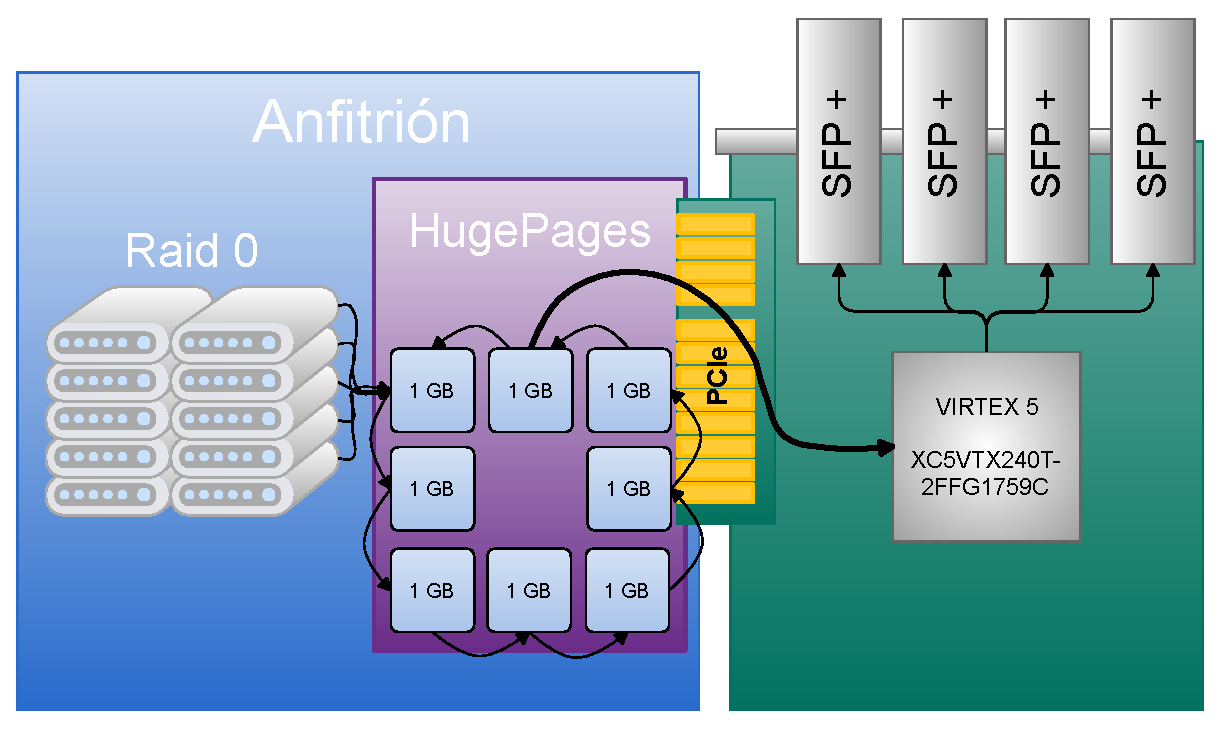
\includegraphics[scale=.6]{rafaDagda}
\caption{Arquitectura del emisor de tráfico}
\label{fig:dis:dpdkdd}
\end{figure}

\begin{figure}[!htb]
\centering
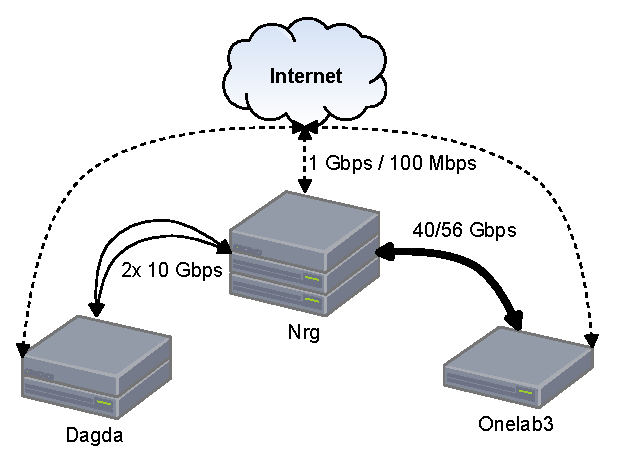
\includegraphics[scale=.8]{conexiones}
\caption{Conexionado del equipo de captura y desarrollo}
\label{fig:dis:dpdkdd}
\end{figure}


\subsubsection{Tráfico emitido}

\subsection{Software utilizado\label{sec:sw}}

\lsection{Metodología de las pruebas\label{sec:metod}}

\lsection{Pruebas en entorno físico\label{sec:fisico}}

\lsection{Pruebas en entornos virtuales\label{sec:virtual}}

\subsection{Usando Passthrough\label{sec:pt}}

\subsection{Usando SR-IOV\label{sec:sriov}}